%# -*- coding: utf-8-unix -*-
%%==================================================
%% tech.tex for SJTU Master Thesis
%%==================================================

%\bibliographystyle{sjtu2}%[此处用于每章都生产参考文献]
\chapter{相关技术分析}
\label{chap:tech}

本章主要介绍了Fornax使用到的技术与工具,其中包括但不限于Docker,Kubernetes。Docker是目前较为流行的容器虚拟化工具,相比于其他的工具,Docker解决了容器从打包,存放,与运行的全流程问题,因此被广为接受,Fornax使用Docker来进行构建环境的搭建与隔离。Kubernetes是由谷歌开源的容器集群管理工具,Fornax基于该工具来进行持续部署。

\section{Docker容器技术}

Docker是一个开源的容器虚拟化工具,它可以帮助开发者便捷地进行容器的构建,发布,与运行。本部分将从容器技术本身,Docker的核心概念,以及Docker的架构,相比于其他容器的工具而言的优势四个部分来介绍Docker这一容器虚拟化工具。

\subsection{容器虚拟化技术概览}

\begin{figure}[!htp]
  \centering
  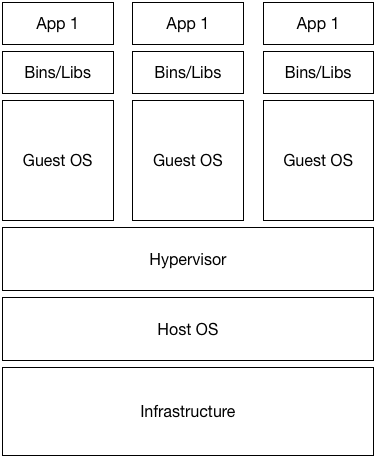
\includegraphics[width=0.4\textwidth]{tech/vm.png}
  \bicaption[fig:vm]{传统虚拟化技术示意图}{传统虚拟化技术示意图}{Fig}{}
\end{figure}

容器虚拟化技术并不是一个最近才出现的新技术,而是在2000年左右就已经有不少应用的虚拟化手段。

在容器虚拟化技术之前,比较常用的虚拟化工具有Xen,VMware等等。这些虚拟化工具都是属于Application Binary Interface级别的虚拟化,这样的虚拟化技术允许多个操作系统同时运行在同一套硬件上。这样的实现方式往往需要一个Virtual Machine Monitor,或者称作VMM的系统,来将硬件资源进行虚拟化,将虚拟机运行在虚拟化后的设备上。

而容器虚拟化技术是属于Application Programming Interface级别的虚拟化,每一个虚拟机,也被称为容器,只是操作系统上的一个进程,与普通的进程不同,容器使用namespace等等方式来将资源隔离,使得进程之间互相不感知。\supercite{soltesz2007container}

相比于传统的虚拟化方式,容器虚拟化更加轻量,启动和销毁的速度快,资源消耗少。但与此同时,容器虚拟化也存在一些问题,首先是使用容器虚拟化的技术虚拟出来的容器,共用操作系统的内核。因此如果容器内导致了内核崩溃,那会影响到其他的容器。而使用Xen等技术,一个虚拟机的崩溃对于其他虚拟机而言,不会有任何影响。\supercite{dua2014virtualization}

\subsection{Docker的核心概念}

Docker是目前被广泛接受的一种容器虚拟化工具,其有着其他容器虚拟化工具所不具备的一些优势。Docker原本是DotCloud公司的一个内部项目,DotCloud是一个专注于平台即服务的创业公司。在2013年3月13日,Docker发布了它的开源版本。它使用了内核中的lxc作为其容器的支持,同时还使用了内核中的cgroups和namespace的特性,因此需要内核支持。在Docker开源后,因为其便捷和高效的特性,受到了开发者的欢迎。在最初的版本中,Docker的网络等方面还不是特别的完善,但是Docker由DotCloud公司进行积极的开发和维护,在2014年的0.9版本中,Docker移除了lxc的依赖,直接与内核中的特性进行交互。并且亚马逊、IBM、微软Azure等等国际云服务提供商纷纷表示将整合Docker技术到其云计算产品中,一时之间Docker成为了云计算领域的热词。截止至2016年5月16日,Docker在Github上收获了31256个关注(Star),成为了Github上最受欢迎的项目之一。

\begin{figure}[!htp]
  \centering
  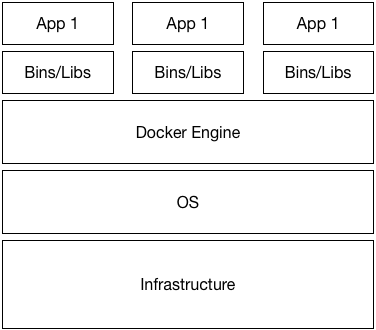
\includegraphics[width=0.4\textwidth]{tech/container.png}
  \bicaption[fig:container]{Docker示意图}{Docker示意图}{Fig}{}
\end{figure}

如图\ref{fig:container}所示,Docker不同于传统的虚拟化技术,每一个容器包含其运行时需要的所有依赖以及应用,但并不需要一个虚拟机来提供支持,每一个Docker容器只是一个运行在独立的namespace下的受到隔离的进程。与此同时,Docker容器不会跟下层的操作系统相耦合,它们可以运行在所有支持Docker Engine的机器或者云上。

Docker中比较重要的两个概念分别是镜像和容器,这是Docker最主要的两个实体概念。镜像是Docker的一个特色,镜像是一个只读的模板,在启动容器时被加载。镜像在存储方面,采取了联合文件系统。联合文件系统允许系统的文件和目录以分层的方式存储,而对于操作系统而言,其使用的文件系统是分层叠加之后的结果。这样使得镜像的存储变得更加方便,可以将不同的文件分层并行地进行上传或下载。而且当对镜像进行修改时,只需要对修改之后的文件分层进行添加或者修改即可,而不需要替换掉整个镜像。而Docker通过定义了一系列操作,将镜像的构建进行了标准化,使得用户只需要通过简单地操作,即可构建出满足自己需要的镜像。

而容器则是镜像的运行时,镜像为容器提供了启动的环境,而容器则与常规的容器虚拟化技术中的容器概念一致,是一个隔离的进程。因为Docker的镜像是一个只读的模板,其所有的文件分层都是设置为只读的,因此当从一个镜像运行起一个容器时,Docker会在镜像的最上层添加一个可读可写的新的文件分层。在新的文件分层中对于文件系统的修改,会覆盖原本的镜像。这样就使得容器看起来运行在镜像之上,而并不会因为容器的运行修改镜像的内容。

\subsection{Docker的架构}

\begin{figure}[!htp]
  \centering
  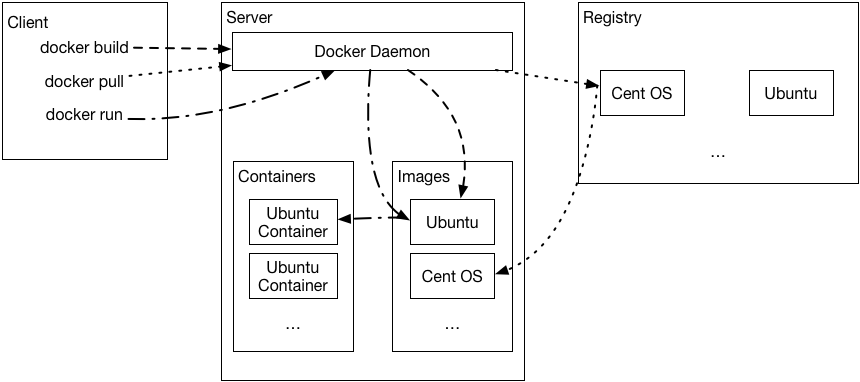
\includegraphics[width=\textwidth]{tech/architecture.png}
  \bicaption[fig:architecture]{Docker架构图}{Docker架构图}{Fig}{}
\end{figure}

如图\ref{fig:architecture}所示,Docker采取了客户端-服务器的架构。其中比较重要的组件有Docker Daemon,Docker Client,Docker Registry三个,下面将从镜像和容器的生命周期角度,对Docker的架构进行介绍。

Docker Daemon,是运行在服务器端的后台程序。其承担了基本所有的操作,包括本地镜像和容器的管理,与远端的Docker Registry的交互等等。但用户并不直接与Docker Daemon交互,而是通过Docker Client。Docker Client是一个Cli程序,为用户提供了抽象度很高的命令,通过Docker Client,用户可以与Docker的服务器进行交互,进而管理容器和镜像。而Docker Registry是管理镜像的存储组件,用户可以将构建好的镜像推送至Docker Registry中,而通过Docker Client,用户可以对Docker Registry上的镜像进行简单的搜索,寻找适合自己应用场景的镜像,并拉取使用。

\subsection{Docker的优势}

Docker有一系列优秀的特性。首先,作为一个容器虚拟化工具,它允许用户创建Docker容器,并且利用iptable等等特性,解决了容器与容器之间互相连接的问题。同时,Docker允许构建镜像,并且可以将镜像推送给远端的Registry,这使得一次构建,多次运行的想法成为了现实。而且Docker的Registry允许多租户,通过类似Github的方式来进行组织与构建,使得Docker在生产环境的使用成为了可能。

除此之外,Docker的成功也离不开其强大的生态环境。围绕着Docker,有一系列工具和技术覆盖了当下很多领域的难题。首先,Docker周边有非常多为了降低Docker的使用门槛的工具,比如Docker Machine等。原本因为容器虚拟化技术需要依赖Linux内核的某些特性,使得其他系统的用户不能使用Docker来构建容器,但是Docker Machine会在非Linux环境下运行一个Linux虚拟机,将Docker运行在该虚拟机上,这抹平了Docker对内核的要求,使得其他系统的用户也可以自如地使用Docker来构建容器,目前Docker正在积极基于OS X的新特性积极地进行对OS X系统的原生支持,这对于OS X系统的用户而言是一大利好。其次,Docker跨平台的特性,使得企业的混合云部署变成了现实。面对当下异构的机器和网络环境,Docker能够更好地发挥其特性。除此之外,在持续集成与持续部署方面,Docker非常用来做环境的隔离,执行构建任务。Drone等工具就是专注于该领域的,基于Docker来实现的工具。
